\documentclass[english]{beamer}

% generated by Docutils <http://docutils.sourceforge.net/>
\usepackage{fixltx2e} % LaTeX patches, \textsubscript
\usepackage{cmap} % fix search and cut-and-paste in PDF
\usepackage{babel}
\usepackage[T1]{fontenc}
\usepackage[latin1]{inputenc}
\usepackage{listings}
\usepackage{amsmath}
\lstset{
  language=TeX,
  basicstyle=\small\ttfamily,
  commentstyle=\ttfamily\color{blue},
  stringstyle=\ttfamily\color{orange},
  showstringspaces=false,
  breaklines=true,
  postbreak = \space\dots
}

\usepackage{ifthen}
\usepackage{longtable}
\usepackage{array}
\setlength{\extrarowheight}{2pt}
\newlength{\DUtablewidth} % internal use in tables

\mode<presentation>
{
  \usetheme{Warsaw}
  \useoutertheme{infolines}
  \setbeamercovered{transparent}
}


\title{\LaTeX}
\author[FOSSEE] {FOSSEE}
\institute[IIT Bombay] {Department of Aerospace Engineering\\IIT
  Bombay}
\date{}

%% Delete this, if you do not want the table of contents to pop up at
%% the beginning of each subsection:
\AtBeginSubsection[]
{
  \begin{frame}<beamer>
    \frametitle{Outline}
    \tableofcontents[currentsection,currentsubsection]
  \end{frame}
}

\AtBeginSection[]
{
  \begin{frame}<beamer>
    \frametitle{Outline}
    \tableofcontents[currentsection,currentsubsection]
  \end{frame}
}

\begin{document}

% Document title
\begin{frame}
  \maketitle  
\end{frame}

\section{Introduction}

\begin{frame}
  \frametitle{\LaTeX~- Introduction}
  \begin{itemize}
  \item Typesetting program
  \item Excellently Typeset Documents - specially Math
  \item Anything from one page articles to books. 
  \item Based on \TeX
  \item Pronounced ``Lah-tech'' or ``Lay-tech''
  \end{itemize}
\end{frame}

\begin{frame}
  \frametitle{This Course}
  \begin{itemize}
  \item Look at Sample document - \texttt{sample.pdf}
  \item The document will be produced by the end of the course. 
  \item First Hour - Basic Structure
  \item Second Hour - Text, Tables, Figures, References
  \item Third Hour - Math, Bibliography, Presentations
  \end{itemize}
\end{frame}


\begin{frame}
  \frametitle{A Look at the Sample Document}
  \begin{itemize}
  \item Title, Author, Date
  \item Abstract
  \item Sections
  \item Subsections
  \item Appendix
  \item References/Bibliography
  \item Tables
  \item Figures
  \item Math
  \end{itemize}
\end{frame}

\begin{frame}[fragile]
  \frametitle{The source \& compilation}
  Write the following code into the file \texttt{draft.tex}.
  \begin{lstlisting}
    \documentclass{article}
    \begin{document}
    SciPy is open-source software for mathematics, 
    science, and engineering.   
    \end{document}
  \end{lstlisting}
  To compile the document, do the following in your terminal: 
  \begin{lstlisting}[language=bash]
    $ pdflatex draft.tex
  \end{lstlisting}
  This produces the output file \texttt{draft.pdf} %%$
  Note: \texttt{latex} command is often used to get \texttt{dvi}
  output. Throughout this course, we shall use \texttt{pdflatex} to
  compile our documents to \texttt{pdf} output.
\end{frame}  

\section{Structure of the Document}

\begin{frame}[fragile]
  \frametitle{\lstinline+documentclass+}
  \begin{itemize}
  \item \LaTeX~typesets based on \lstinline{documentclass}
  \item Defines structure and formatting of a document
  \item \LaTeX~is a document based mark-up
  \item Mark-up --- a system of annotating text, adding extra
    information to specify structure and presentation of text
  \item Document based markup $\rightarrow$ you don't have to worry
    about each element individually 
  \item Allows you to focus on content, rather than appearance.
  \end{itemize}
\end{frame}

\begin{frame}[fragile]
  \frametitle{Environments and Commands}
  \lstinline{document} is an environment, present in every document. 
  \begin{itemize}
  \item Environments
    \begin{itemize}
    \item \lstinline{\begin} and \lstinline{\end} define the beginning
      and end of an environment
    \item All the content of the document is placed inside the
      \lstinline{document} environment 
    \end{itemize}
  \item Commands
    \begin{itemize}
    \item All commands begin with \textbackslash
    \item They are case-sensitive
    \item Only alpha caracthers; other characters terminate commands
    \end{itemize}
  \end{itemize}
\end{frame}


\begin{frame}[fragile]
  \frametitle{Top Matter}
  Let's add the Title, Author's name and the date to the document.
  \begin{itemize}
  \item Add title, author and date. Compile. Nothing changes.
  \end{itemize}
  \begin{lstlisting}
    \title{A Glimpse at Scipy}
    \author{FOSSEE}
    \date{June 2010}
  \end{lstlisting}
  \tiny{See \texttt{hg} rev1 of draft.}
\end{frame}

\begin{frame}[fragile]
  \frametitle{Top Matter \ldots}
  \begin{itemize}
  \item \lstinline{\maketitle} command inserts the top-matter.
  \item Compile again. 
  \item If no date is specified, today's date is automatically
    inserted.
  \end{itemize}
  \begin{lstlisting}
    \begin{document}
    \maketitle
    SciPy is open-source software for mathematics, science, and engineering.   
    \end{document}
   \end{lstlisting}
  \tiny{See \texttt{hg} rev2 of draft.}
\end{frame}


\begin{frame}[fragile]
  \frametitle{Abstract}
  \begin{itemize}
  \item The abstract environment is placed at the location where it's
    put in the source. 
  \end{itemize}
  \begin{lstlisting}
    \begin{abstract}
      This document shows a glimpse of the features of Scipy that will
      be explored during this course.
    \end{abstract}
  \end{lstlisting}
  \tiny See rev3 of \texttt{hg}
\end{frame}

\begin{frame}[fragile]
  \frametitle{Sectioning}
  \begin{itemize}
  \item \lstinline{\section}, \lstinline{\subsection}
    \lstinline{\subsubsection}
  \item Auto numbered sections!
  \item \* to prevent numbering of a section
  \end{itemize}
  \begin{lstlisting}
    \section{A Glimpse of Scipy functions}
    \subsection{Matrix Operations}
    \subsubsection{Inverse}
  \end{lstlisting}
  \tiny See rev4 of \texttt{hg}
\end{frame}

\begin{frame}[fragile]
  \frametitle{Sectioning \ldots}
  \begin{itemize}
  \item Longer documents, use \lstinline{report} or \lstinline{book}
    class
  \item Chapter can be added using \lstinline{\chapter}
  \end{itemize}
  \begin{lstlisting}
    \documentclass{report}

    \chapter{One}
  \end{lstlisting}
  \begin{itemize}
  \item subsections do not get numbering
  \item Change \lstinline{secnumdepth}
  \end{itemize}
  \begin{lstlisting}
    \setcounter{secnumdepth}{3}
  \end{lstlisting}
   \tiny See rev5 of \texttt{hg}
\end{frame}

\begin{frame}[fragile]
  \frametitle{Appendices}
  \begin{itemize}
  \item Anything following the \lstinline{\appendix} command is added
    to the Appendix. 
  \end{itemize}
  \begin{lstlisting}
    \appendix
    
    \section{Plotting using Pylab}
  \end{lstlisting}
  \tiny See rev7 of \texttt{hg}
\end{frame}

\begin{frame}[fragile]
  \frametitle{Table of Contents [TOC]}
  \begin{itemize}
  \item Our document is short, but let's learn to add a TOC.
  \item Add \lstinline{\tableofcontents} where you want TOC to
    appear.
  \item Compile. 
  \item Only headings appear. No page numbers. 
  \item A \lstinline{.toc} file is generated. 
  \item Re-compile.
  \item Any numbered section/block automatically appears
  \end{itemize}
  \tiny See rev8 of \texttt{hg}
\end{frame}

\begin{frame}[fragile]
  \frametitle{TOC \ldots}
  \begin{itemize}
  \item To add un-numbered sections, use \lstinline{\addcontentsline}
  \end{itemize}
  \begin{lstlisting}
    \section*{Introduction}
    \addcontentsline{toc}{section}{Intro}
  \end{lstlisting}
  \tiny See rev9 of \texttt{hg}
\end{frame}

\begin{frame}
  \frametitle{Bibliography}
  We shall look at Bibliographies, later in the course. 
\end{frame}

\section{Typesetting Text}
\begin{frame}[fragile]
  \frametitle{Line breaks, Paragraphs}
  \begin{itemize}
  \item Add the text of second paragraph in the introduction section. 
  \item Compile. 
  \item An empty line starts a new para
  \item New paragraphs are indented
  \item Multiple spaces or empty lines are considered as one
  \item To start a new line \lstinline{\\} or \lstinline{\newline}
  \end{itemize}
  \tiny See rev10 of \texttt{hg}
\end{frame}

\begin{frame}[fragile]
  \frametitle{Quotation Marks}
  \begin{itemize}
  \item The quotation marks around Sigh Pie are not formatted properly
  \item Use \`~ (accent) for left quote
  \item Use \'~ (apostrophe) for right quote
  \item For double quotes, use them twice
  \end{itemize}
  \begin{center}
    \`~\`~Sigh Pie\'~\'~
  \end{center}
  \tiny See rev11 of \texttt{hg}
\end{frame}

\begin{frame}[fragile]
  \frametitle{Fonts - Emphasis, Fixed width, \ldots}
  \begin{itemize}
  \item \lstinline{\emph} gives emphasized or italic text
  \item \LaTeX environments can be nested
  \item Let's add sub-package names as text, before learning to
    typeset tables
  \item Note multiple spacing won't work
  \end{itemize}
  \begin{lstlisting}
    Subpackage - Description\\
    cluster - Clustering algorithms\\
    constants - Physical and mathematical constants\\
    fftpack - Fast Fourier Transform routines\\
  \end{lstlisting}
  \begin{center}
    \hspace{1in}\vdots
  \end{center}
  \tiny See rev12 of \texttt{hg}
\end{frame}

\begin{frame}[fragile]
  \frametitle{Fonts - Emphasis, Fixed width, \ldots}
  \begin{itemize}
  \item Use \lstinline{\texttt} for sub-packages names - fixed width
  \item \lstinline{\textbf} for bold face
  \item \lstinline{-} can be replaced with \lstinline{--} or
    \lstinline{---} for better formatting
  \end{itemize}
  \begin{lstlisting}
    \textbf{Subpackage} --- \textbf{Description}\\
    \texttt{cluster} --- Clustering algorithms\\
    \texttt{constants} --- Physical and mathematical constants\\
    \texttt{fftpack} --- Fast Fourier Transform routines\\
  \end{lstlisting}
  \begin{center}
    \hspace{1in}\vdots
  \end{center}
  \tiny See rev13 of \texttt{hg}
\end{frame}

\subsection{Lists}
\begin{frame}[fragile]
  \frametitle{Lists}
  \begin{itemize}
  \item \lstinline{enumerate} environment is used for numbered lists
  \item \lstinline{itemize} environment gives un-numbered lists
  \item Each item in the list is specified using \lstinline{\item}
  \item Nested lists are also easily handled, as expected
  \item Example on next slide
  \end{itemize}
  \tiny See rev14 of \texttt{hg}
\end{frame}

\begin{frame}[fragile]
  \frametitle{Lists \ldots}
  \begin{lstlisting}
    \begin{enumerate}
    \item Plotting
    \item Matrix Operations
      \begin{itemize}
      \item Inverse
      \end{itemize}
    \item Solving Equations
      \begin{itemize}
      \item System of Linear equations
      \end{itemize}
    \item Integration 
      \begin{itemize}
      \item Quadrature
      \item ODEs
      \end{itemize}
    \end{enumerate}
  \end{lstlisting}
\end{frame}

\begin{frame}[fragile]
  \frametitle{Footnotes}
  \begin{itemize}
  \item Add footnote for \lstinline{pylab}
  \item It's easily done using \lstinline{\footnote} command 
  \end{itemize}
  \begin{lstlisting}
    Plotting \footnote{using \texttt{pylab} - see Appendix A} 
  \end{lstlisting}
  \begin{itemize}
  \item We have just written down the name of the appendix
  \item But if another section is added before it, the reference has
    to be changed
  \item \LaTeX provides labels and references
  \end{itemize}
  \tiny See rev15 of \texttt{hg}
\end{frame}

\begin{frame}[fragile]
  \frametitle{Labels and References}
  \begin{itemize}
  \item First add a label to the section that we wish to refer to
  \item \lstinline+\label{labelname}+
  \item Change footnote to use the reference
  \item \lstinline+\ref{labelname}+
  \item Compile twice
  \end{itemize}
  \begin{lstlisting}
    \section{Plotting using Pylab}\label{mpl}

    Plotting \footnote{using \texttt{pylab} - see Appendix \ref{mpl}} 
  \end{lstlisting}
  \tiny See rev15 of \texttt{hg}
\end{frame}

\begin{frame}[fragile]
  \frametitle{Including code}
  \begin{itemize}
  \item Instead of using \lstinline{\texttt} we could use
    \lstinline{\verbatim} 
  \item \lstinline{listings} is a powerful package
  \item \lstinline+\usepackage{listings}+ needs to be added 
  \item Tell \LaTeX the language, you are going to use
  \end{itemize}
  \begin{lstlisting}
    \usepackage{listings} 
    \lstset{language=Python,
      basicstyle=\ttfamily\bfseries,
      showstringspaces=false}
  \end{lstlisting}
  \tiny See rev16 of \texttt{hg}
\end{frame}

\begin{frame}[fragile]
  \frametitle{Including code}
  \begin{itemize}
  \item Use \lstinline{lstlisting} for a block of code
  \item \lstinline+\lstinline+ for inline code
  \item Let's add the code to Appendix
  \end{itemize}
  \begin{lstlisting}
    \begin{lstlisting.}
      In []: x = linspace(0, 2*pi, 50)
      In []: plot(x, sin(x))
      In []: title('Sine Curve between 0 and $\pi$')
      In []: legend(['sin(x)'])
    \end{lstlisting.}
  \end{lstlisting}
  \tiny See rev16 of \texttt{hg}
\end{frame}

\section{Figures, Tables \& Floats}
\begin{frame}[fragile]
  \frametitle{Figures}
  \begin{itemize}
  \item Let's add the figure in the Appendix
  \item \lstinline+\usepackage{graphicx}+
  \item To add a graphic, use \lstinline{\includegraphics} command
  \item We give the relative path to the \lstinline+.png+ image
  \end{itemize}
  \begin{lstlisting}
    \usepackage{graphicx}
    
    \begin{figure}[h!]
    \begin{center}
      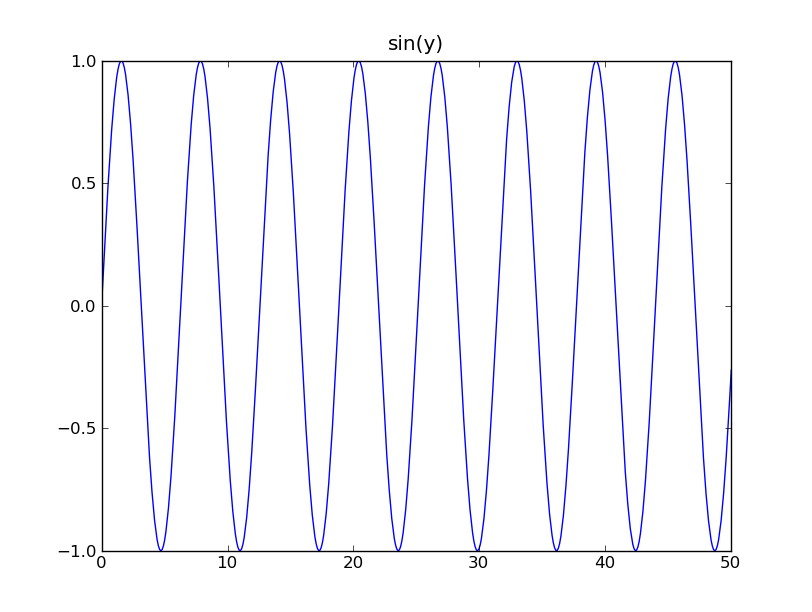
\includegraphics[scale=0.4]{../sine.png}      
    \end{center}
    \caption{Sine Curve}
    \label{fig:sin}
    \end{figure}
  \end{lstlisting}

  \tiny See rev17 of \texttt{hg}
\end{frame}

\begin{frame}[fragile]
  \frametitle{\lstinline{includgraphics}}
  It takes following optional arguments
  \begin{itemize}
  \item \lstinline+scale+ --- specifies the factor by which to scale
    the image 
  \item \lstinline+height+, \lstinline+width+ --- If only one of them
    is specified, aspect ratio is maintained 
  \item \lstinline+keepaspectratio+ --- boolean value to keep aspect
    ratio or not 
  \item \lstinline+angle+ --- specify by what angle the image should
    be rotated 
  \end{itemize}
\end{frame}

\begin{frame}[fragile]
  \frametitle{Floats}
  \begin{itemize}
  \item Graphics (\& Tables) are special because they cannot be broken
    across pages 
  \item They are ``floated'' to the next page, if they don't fit in
    the current page 
  \item Enclose graphic within \lstinline+figure+ environment to make
    it float 
  \item Figure environment takes additional parameter for location of
    float 
  \end{itemize}
  \begin{table}
    \caption{Permission Specifiers}
    
    \begin{tabular}{|c|c|}
      Specifier & Permission\\\hline
      t & Top of page\\
      b & Bottom of page\\
      p & Separate page for floats\\
      h & here (the same place where command appears in source)\\
      ! & override \LaTeX's internal parameters for good position
    \end{tabular}
  \end{table}
\end{frame}

\begin{frame}
  \frametitle{Captions and References}
  \begin{itemize}
  \item Figure environment allows us add a caption
  \item To place the image in the center we enclose it in the
    \lstinline+center+ environment 
  \item We can label images too
  \item label shoule be added after the caption command
  \item Figures are auto numbered
  \end{itemize}
  \tiny See rev17 of \texttt{hg}
\end{frame}

\subsection{Tables}

\begin{frame}[frame]
  \frametitle{Tables}
  \begin{itemize}
  \item \lstinline+tabular+ is used to typeset a table
  \item It is enclosed in a \lstinline+table+ environment to make it a
    float 
  \item \lstinline+table+ environment also gives captions, auto
    numbering  
  \end{itemize}
\end{frame}


\begin{frame}[fragile]
  \frametitle{\lstinline+tabular+}
  \begin{itemize}
  \item tabular takes formatting of each column as argument
  \end{itemize}

  \begin{table}
    \caption{tabular environment}
    
    \begin{tabular}{|l|l|}
      \lstinline+l+ & left justified column content\\\hline
      \lstinline+r+ & right justified column content\\\hline
      \lstinline+c+ & centered column content\\\hline
      \lstinline+|+ & produces a vertical line\\
    \end{tabular}
  \end{table}
  \begin{itemize}
  \item also takes an optional parameter for specifying position of
    table 
  \item \lstinline+t+ for top, \lstinline+b+ for bottom, \lstinline+c+
    for center 
  \item each column of table is separated by \&
  \item each row is separated by newline \lstinline{\\}
  \item \lstinline+\hline+ give a horizontal line between two rows
  \end{itemize}
  \tiny See rev18 of \texttt{hg}
\end{frame}

\begin{frame}[fragile]
  \frametitle{\lstinline+tabular+ \ldots}
  \begin{lstlisting}
    \begin{table}
      \caption{Sub-packages available in Scipy}
      \label{subpkg}
      \begin{tabular}{|l|l|}
        \hline
        \textbf{Subpackage} & \textbf{Description}\\
        \texttt{constants} & Physical and mathematical constants\\
        \hline
        \texttt{fftpack} & Fast Fourier Transform routines\\
        \hline
        \end{tabular}
      \end{table}
    \end{lstlisting}
\end{frame}

\begin{frame}[fragile]
  \frametitle{List of Tables, Figures}
  \begin{itemize}
  \item \lstinline+listoftables+
  \item \lstinline+listoffigures+
  \end{itemize}
\end{frame}


\section{Typesetting Math}
\begin{frame}[fragile]
  \frametitle{Math in \LaTeX}
  \begin{itemize}
  \item Math is enclosed in a pair of \lstinline{$} signs o
    \lstinline+\(  \)+ %$
  \item Used for typesetting inline Math. 
  \item \lstinline+\usepackage{amsmath}+
  \item Let's now move on to matrices. 
  \end{itemize}
\end{frame}

\begin{frame}[fragile]
  \frametitle{Matrices}
  \begin{itemize}
  \item \lstinline+\bmatrix+ is used to typeset the matrix A
  \item It works similar to ta tabular environment
  \item \lstinline+&+ for demarcating columns
  \item \lstinline+\\+ for demwarcating rows
  \end{itemize}
  \begin{lstlisting}
    Let $\mathbf{A}$ be the matrix 
    \(
    \begin{bmatrix}
      1 &3 &5\\
      2 &5 &1\\
      2 &3 &8
    \end{bmatrix}
    \)
  \end{lstlisting}
  \tiny See rev19 of \texttt{hg}    
\end{frame}

\begin{frame}[fragile]
  \frametitle{Matrices \ldots}
  \begin{itemize}
  \item There are 5 other matrix environments 
  \end{itemize}
  \begin{table}
    \center
    \begin{tabular}{c|c}
      \lstinline+matrix+  &  none\\
      \lstinline+pmatrix+ &  \lstinline+(+\\
      \lstinline+Bmatrix+ &  \lstinline+{+\\
        \lstinline+vmatrix+ &  \lstinline+|+\\  
        \lstinline+Vmatrix+ &  \lstinline+||+
    \end{tabular}
  \end{table}
\end{frame}

\begin{frame}[fragile]
  \frametitle{Superscripts \& Subscripts}
  \begin{itemize}
  \item \lstinline+^+ for superscripts
  \item To have multiple characters as sub/superscript, enclose in
    \lstinline+{ }+
  \item \lstinline+_+ for subscripts
  \end{itemize}
\end{frame}

\begin{frame}[fragile]
  \frametitle{Summation \& integration}
  \begin{itemize}
  \item \lstinline+\sum+ command gives the summation symbol
  \item The upper and lower limits are specified using the
    \lstinline+^+ and \lstinline+_+ symbols. 
  \item Similarly the integral symbol is obtained using
    \lstinline+\int+ command. 
  \end{itemize}
\end{frame}

\begin{frame}[fragile]
  \frametitle{\lstinline+displayed+ math}
  \begin{itemize}
  \item The equation in Determinants section is different. 
  \item It is a displayed equation. 
  \item \LaTeX~ or \lstinline+amsmath+ has a number of environments
    for ``displaying'' equations, with minor differences. 
  \item In general, enclose math in \lstinline+\[+ and \lstinline+\]+
    to get displayed math. 
  \item \lstinline+\begin*{equation}+ is equivalent to this.
  \item Use \lstinline+\begin{equation}+ to get numbered
    equations. %%\end{equation} 
  \end{itemize}
  \begin{lstlisting}
    \[ \left|\mathbf{A}\right|=\sum_{j}\left(-1\right)^{i+j}a_{ij}\mathbf{M}_{ij} \]
  \end{lstlisting}
  \tiny See rev20 of \texttt{hg}    
\end{frame}

\begin{frame}[fragile]
  \frametitle{Groups of equations}
  \begin{itemize}
  \item The \lstinline+equation+ environment allows typesetting of
    just 1 equation. 
  \item \lstinline+eqnarray+ allows typesetting of multiple equations 
  \item It is similar to the \lstinline+table+ environment
  \item The parts of the equation that need to be aligned are
    indicated using \& symbol.
  \item Each equation is separated by a \lstinline+\newline+ command
  \end{itemize}
  \begin{lstlisting}
    \begin{eqnarray*}
      x^3 - 2x^2 - \frac{1}{2}x + 1 = 0\\
      x^2(x-2) - \frac{1}{2}(x-2) = 0\\
      (x-2)(x^2 - \frac{1}{2}) = 0\\
      (x-2)(x - \frac{1}{\sqrt{2}})(x + \frac{1}{\sqrt{2}}) = 0
    \end{eqnarray*}    
  \end{lstlisting}
  \tiny See rev21, 22 of \texttt{hg}    
\end{frame}

\begin{frame}[fragile]
  \frametitle{Fractions \& Surds}
  \begin{itemize}
  \item Fractions are typeset using \lstinline+\frac+ command 
  \item \lstinline+\frac{numerator}{denominator}+ is typeset as
    $\frac{numerator}{denominator}$
  \item Surds are typeset using \lstinline+\sqrt[n]+ command
  \end{itemize}
\end{frame}

\begin{frame}[fragile]
  \frametitle{Greek characters \& Spacing}
  \begin{itemize}
  \item Typesetting Greek characters is simple
  \item \lstinline+\alpha+, \lstinline+\beta+, \lstinline+\gamma+,
    \ldots \lstinline+\Alpha+, \lstinline+\Beta+, \lstinline+\Gamma+
    \ldots 
  \item To get additional spacing in Math environments ---
\begin{center}
\begin{tabular}{|l|l|l|}
\hline
 Abbrev. & Spelled out & Example  \\
\hline
 \lstinline+\,+ & \lstinline+\thinspace+ & $A\,B$ \\
\hline
 \lstinline+\:+ & \lstinline+\medspace+ & $A\:B$ \\
\hline
 \lstinline+\;+ & \lstinline+\thickspace+ & $A\;B$ \\
\hline
   & \lstinline+\quad+ & $A \quad B$ \\
\hline
   & \lstinline+\qquad+ & $A \qquad B$ \\
\hline
 \lstinline+\!+ & \lstinline+\negthinspace+ & $A!B$ \\
\hline
   & \lstinline+\negmedspace+ & $A \negmedspace B$ \\
\hline
   & \lstinline+\negthickspace+ & $A \negthickspace B$ \\
\hline

\end{tabular}
\end{center}
  \end{itemize}
\end{frame}

\section{Bibliography}
\begin{frame}[fragile]
  \frametitle{Bibliography}
  \begin{itemize}
  \item \lstinline+thebibliography+ environment provides a clean and
    simple way to add a bibliography to \LaTeX documents. 
  \item \lstinline+\begin{thebibliography}+ takes as argument the
    maximum with of the label that references will have. 
  \item Each item of the Bibliography is similar to an item in a
    list. 
  \item \lstinline+\bibitem[label]{name}+ followed by the actual
    reference info. 
  \item label replaces auto enumeration numbers 
  \item \lstinline+\cite{name}+ is used to \lstinline+cite+ the
    \lstinline+bibitem+ 
  \item You will need to compile twice. 
  \end{itemize}
\end{frame}

\begin{frame}[fragile]
  \frametitle{Bibliography}
  \begin{lstlisting}
    \begin{thebibliography}{9}
    \bibitem{scipy} 
      Eric Jones and Travis Oliphant and Pearu Peterson and others,
      \emph{SciPy: Open source scientific tools for Python}, 2001 -- , 
      \url{http://www.scipy.org/} 
  \end{lstlisting}
  \tiny See rev23 of \texttt{hg}    
\end{frame}

\section{Presentations - Beamer}
\begin{frame}[fragile]
  \frametitle{Beamer}
  \begin{itemize}
  \item Use beamer since your report's \LaTeX~ would be re-usable.
  \item It is recommended to start with on of the beamer templates.
  \item Let's look at speaker introduction template.
  \item \lstinline+\documentclass{beamer}+ tells \LaTeX~ to start a
    beamer presentation. 
  \item A beamer document is very similar to any other \LaTeX~
    document except that content is divided into slides. 
  \end{itemize}
\end{frame}

\begin{frame}[fragile]
  \frametitle{Beamer \ldots}
  \begin{itemize}
  \item \lstinline+\usetheme+ command is used to specify the theme of the
    presentation. 
  \item \lstinline+\usecolortheme+ command is used to specify the color
    theme. 
  \item The content of a slide is enclosed within
    \lstinline+\begin{frame}{Title}{Subtitle}+ and
    \lstinline+\end{frame}+ 
  \item If the slide contains \lstinline+verbatim+
    \lstinline+lstlisting+ environments, the \lstinline+\begin{frame}+
    should be passed an additional argument \lstinline+[fragile]+
  \item Overlays can be achieved using the \lstinline+\pause+
    command. 
  \item To achieve more with beamer, it is highly recommended that you
    look at the \texttt{beameruserguide} 
  \end{itemize}
\end{frame}

\end{document} 
 
